% !TeX root = ../Tempel-Daniel.tex
\chapter{Structured Outputs, Function Calling and Tool Use}
\label{chap:tool-use}


The previous chapter described how candidate models can be evaluated within the intended software-engineering workload. However, selecting a capable model is not sufficient to build the AI Software Engineering Assistant. A language model can generate explanations, code and recommendations, but free-form text alone does not provide a reliable software interface to repositories, test runners, databases or external APIs. The assistant therefore requires mechanisms that turn model generation into machine-readable data and action requests that conventional software components can process.

As described in Chapter~\ref{chap:local-llms}, an LLM still generates tokens autoregressively. Structured output and function calling do not change this basic inference process or give the model direct access to external systems. Instead, they constrain and interpret parts of the generated output so that the model can interact with the surrounding application through defined interfaces.

\section{Structured outputs as a machine-readable interface}
\label{sec:structured-outputs}

A free-form response may express the intended information correctly while still being difficult for software to process reliably. For example, a model could identify \texttt{src/auth.py} as the affected file using many different natural-language formulations. Returning the same information as structured data creates a more explicit interface:

\noindent\begin{minipage}{\linewidth}
\small\singlespacing
\begin{verbatim}
{
  "affected_file": "src/auth.py",
  "needs_fix": true
}
\end{verbatim}
\end{minipage}

JSON provides a machine-readable representation, but syntactically valid JSON alone does not guarantee that an application receives the expected fields and data types. JSON Schema provides a formal vocabulary for describing the structure and validation constraints of JSON documents \parencite{jsonschema2022}. A schema can, for example, require \texttt{affected\_file} to be a string and \texttt{needs\_fix} to be a Boolean.

This distinction also appears in current LLM APIs. JSON mode constrains a response to valid JSON, whereas schema-constrained output additionally constrains its structure to a supplied schema. OpenAI refers to the latter capability as \emph{Structured Outputs} and explicitly distinguishes it from JSON mode \parencite{openai-structured-outputs}.

Schema constraints can be applied during generation rather than only after a complete response has been produced. An inference runtime can restrict candidate output according to a grammar derived from the required structure. The llama.cpp inference runtime introduced in Chapter~\ref{chap:local-llms}, for example, supports GBNF grammars and can convert a supported subset of JSON Schema into such grammars \parencite{ggml-grammars}.

Constraining the output format does not, however, replace instructions describing the intended meaning of its fields. In llama.cpp, a JSON schema used for ordinary constrained output is not automatically visible to the model and must be complemented by an appropriate prompt; tool-calling schemas are handled differently and are supplied as part of the model interaction \parencite{ggml-grammars}.

Structural correctness must therefore be separated from semantic correctness. An argument such as \texttt{"path": "banana.py"} may satisfy a schema requiring a string while still referring to a file that does not exist in the selected repository. Likewise, a schema cannot determine whether inspecting that file is the appropriate action for the current task. Schema-constrained output improves the reliability of the interface, but it does not establish the correctness of the generated values or decisions.

Schema adherence is also separate from successful request completion. A response may remain incomplete because of output limits or inference/API failures, while a refusal may be returned instead of the requested structure. Providers and inference runtimes may additionally support only subsets of the full JSON Schema language. Applications must therefore distinguish request completion, structural validity and semantic validity.

\section{Function calling and tool execution}
\label{sec:function-calling}

Structured output is useful when an application requires structured information. Function calling applies a similar interface to actions. Instead of returning only data, the model can generate a structured request identifying an available operation and the arguments required to invoke it. A request to inspect a source file could conceptually be represented as:

\noindent\begin{minipage}{\linewidth}
\small\singlespacing
\begin{verbatim}
{
  "name": "read_file",
  "arguments": {
    "path": "src/auth.py"
  }
}
\end{verbatim}
\end{minipage}

The corresponding tool definition usually contains a name, description and schema for its arguments. The model therefore receives a description of an available capability rather than the implementation of the underlying function.

Function calling does not by itself guarantee that generated arguments satisfy the declared schema. This depends on the API or inference runtime and the constraint mode being used. OpenAI, for example, distinguishes strict function calling, which enforces the supplied function schema through Structured Outputs, from non-strict best-effort generation \parencite{openai-function-calling}.

The execution boundary is central to the assistant architecture. The LLM does not itself open files, execute tests or call remote APIs. It generates a structured request for an operation. The assistant runtime receives this request, validates its arguments, checks that the requested operation is permitted within the task's allowed scope and dispatches the corresponding software operation. The result is then returned to the runtime and can be included in a subsequent model request.

\noindent\begin{minipage}{\linewidth}
\centering
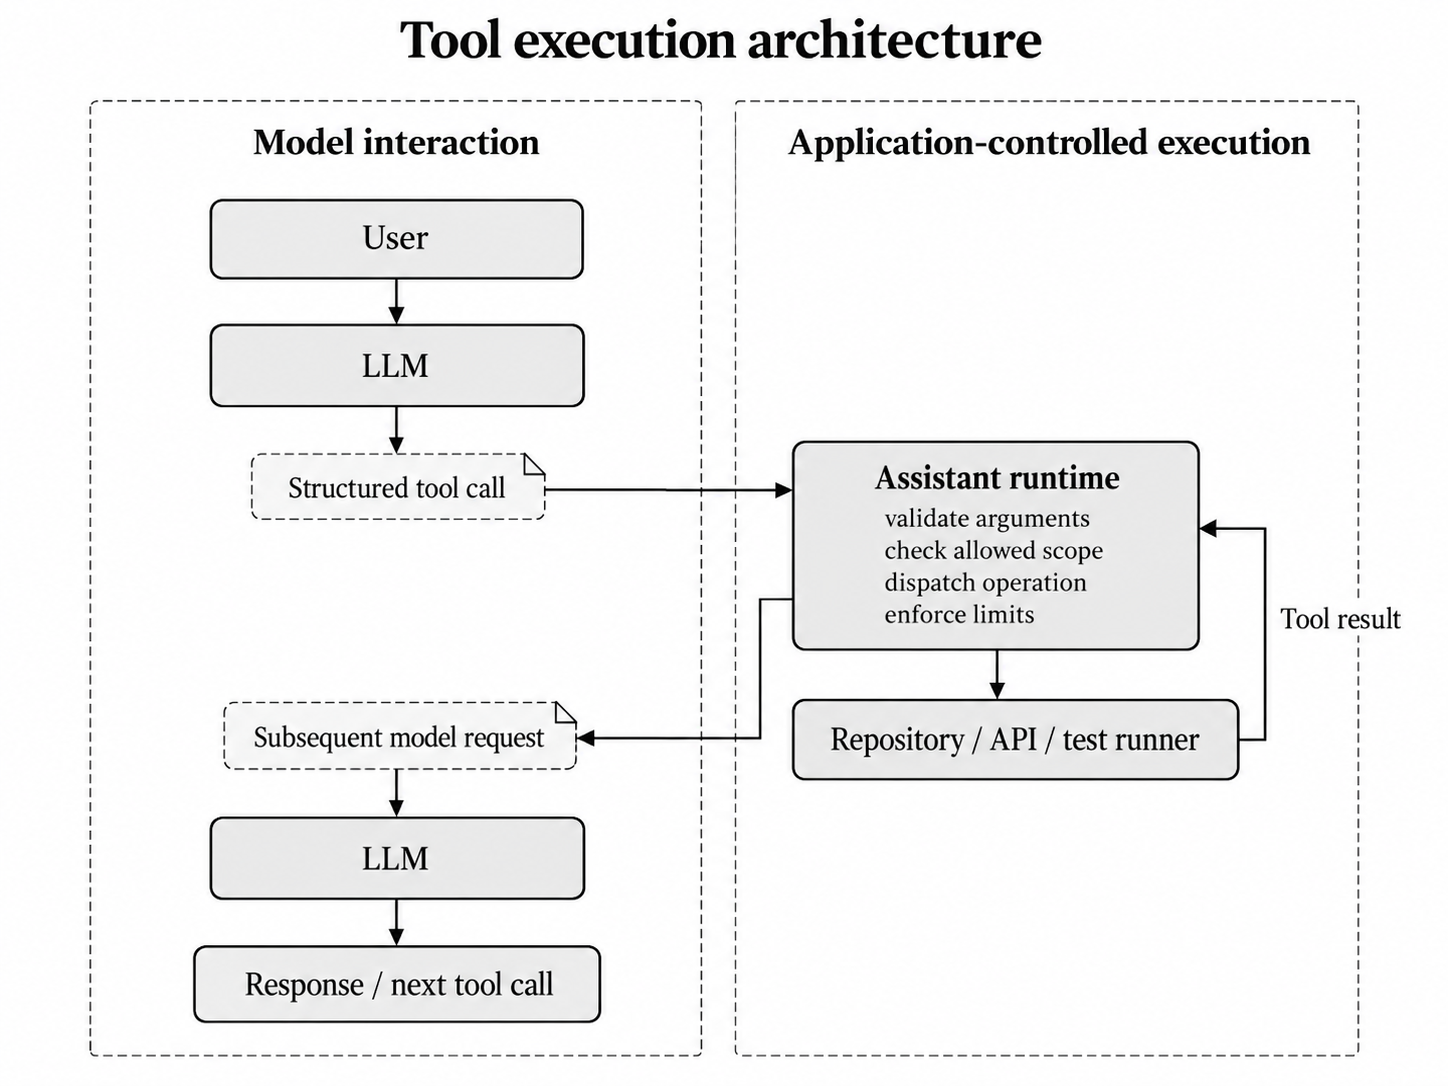
\includegraphics[width=15cm]{images/tool-execution-architecture.png}
\captionsetup{hypcap=false}
\captionof{figure}{Separation between model-generated tool requests and application-controlled tool execution in the AI Software Engineering Assistant.}
\label{fig:tool-execution}
\end{minipage}


This interaction can be summarised as:

\begin{center}
\small\singlespacing
\begin{tabular}{c}
User \\
\(\downarrow\) \\
LLM \\
\(\downarrow\) structured tool call \\
Assistant runtime \\
\(\downarrow\) \\
Repository / API / test runner \\
\(\downarrow\) tool result \\
Assistant runtime \\
\(\downarrow\) subsequent model request \\
LLM \\
\(\downarrow\) \\
response or subsequent tool call \\
\end{tabular}
\end{center}

The execution environment does not necessarily have to be the developer's own process. Some platforms provide tools executed by provider infrastructure, while others return tool requests to the client application for execution. The architectural distinction remains the same: generation specifies an operation, while the actual operation is performed outside the model itself.

Tool results provide new observations that can be included in the model's active context. If \texttt{read\_file} returns the current contents of \texttt{src/auth.py}, the model can reason over that repository state rather than relying on information encoded in its weights. Tool use therefore connects model reasoning to current external state while preserving a software-controlled execution boundary.

\section{Tool interaction and practical constraints}
\label{sec:tool-constraints}

The interaction can be illustrated using the recurring task \emph{Fix GitHub issue \#42 and verify the solution}. The assistant could first request \texttt{get\_issue(42)} to retrieve the current issue description. If the issue refers to missing handling of an \texttt{Authorization} header, the model could then request \texttt{search\_code("Authorization")} followed by \texttt{read\_file("src/auth.py")}. After identifying the required modification, it could request an \texttt{apply\_patch} operation to change the repository and then invoke \texttt{run\_tests(...)} to evaluate the modified state.

This sequence separates generation of a proposed change from its application to the repository. Producing corrected source code does not itself modify a file; the modification occurs only when the corresponding tool operation is executed by the surrounding system.

At each interaction step, several different forms of correctness should be distinguished:

\noindent\begin{minipage}{\linewidth}
\captionsetup{hypcap=false}
\captionof{table}{Levels of correctness in model-generated tool requests.}
\label{tab:tool-failures}
\small\singlespacing
\renewcommand{\arraystretch}{1.15}
\begin{tabular}{@{}p{2.0cm}p{6.5cm}p{7.0cm}@{}}
\toprule
{\raggedright\textbf{Failure level}\par} & \textbf{Question} & \textbf{Example} \\
\midrule
{\raggedright Syntax\par} & {\raggedright Can the generated request be parsed?\par} & {\raggedright Malformed JSON\par} \\
{\raggedright Schema\par} & {\raggedright Does it satisfy the declared tool contract?\par} & {\raggedright Missing required \texttt{path}\par} \\
{\raggedright Semantic\par} & {\raggedright Do the arguments satisfy the operation's preconditions in the current environment?\par} & {\raggedright Requesting a file that does not exist in the selected repository\par} \\
{\raggedright Decision\par} & {\raggedright Is the requested operation appropriate for the task?\par} & {\raggedright Requesting a file modification when the user asked for read-only analysis\par} \\
\bottomrule
\end{tabular}
\end{minipage}

Strict schema-constrained generation can substantially reduce syntax and schema failures, but it cannot establish semantic validity or the quality of the model's action selection. Those properties depend on the current environment, task requirements and model reasoning.

Tool execution can also fail independently of the generated request. A file may have been removed, an external API may return an error or a test process may exceed its execution limit. Rather than hiding such failures, the assistant runtime can return them as structured tool results:

\noindent\begin{minipage}{\linewidth}
\small\singlespacing
\begin{verbatim}
{
  "ok": false,
  "error": "FILE_NOT_FOUND",
  "path": "src/auth.py"
}
\end{verbatim}
\end{minipage}

Such a result can be added to the next model request, allowing the model to revise its next action. Repeated model–tool interaction therefore creates a feedback loop between model-generated decisions and observations obtained through actual tool execution. The runtime can additionally enforce execution limits and determine whether another interaction step is permitted or control should return to the user.

\begingroup
\setlength{\emergencystretch}{2em}
Tool interaction also introduces operational overhead. Tool definitions and argument schemas must be made available to the model, while generated calls and returned results increase the amount of information exchanged across model requests. Multiple model–tool rounds add execution latency, and returned results may increase the active context described in Chapter~\ref{chap:local-llms}.
\par\endgroup

Function calling and tool execution therefore provide the interface through which the AI Software Engineering Assistant can interact with external software, but they do not determine which repository information, previous observations or available capabilities should be presented to the model at a particular step. As the available information grows, selecting and maintaining the relevant active context becomes a separate architectural problem. This is addressed in the following chapter on Context Engineering and Memory.
